% %%%%%%%%%%%%%%%%%%%%%%%%%%%%%%%%%%%%%%%%%%%%%%%%%%%%%%%%%%%%%%%%%%%%%%%%%%%%%
% %%%%%%%%%%%%%%%%%%%%%%%%%%%%%%%%%%%%%%%%%%%%%%%%%%%%%%% Building on Mann 1995
% %%%%%%%%%%%%%%%%%%%%%%%%%%%%%%%%%%%%%%%%%%%%%%%%%%%%%%%%%%%%%%%%%%%%%%%%%%%%%

\chapter{Large Modenumber Effects}
  \label{ch_azm}

\todo{This chapter is the real moneymaker. The overarching motivation for this work is that Pc4 pulsations vary in interesting ways with respect to azimuthal modenumber, and that prior models have been unable to give a good picture of that behavior. }

%\todo{Do we every check E/B against $\Sigma_P / \mz$? }

%\todo{Do we see a difference between \vec{k} (momentum) and the group velocity? Poynting flux will always be pretty much along the field line, since $B_3$ is small and $E_3$ is zero, but the wave vector need not be. This is a question of coupling/converting to compressional waves, I guess. }

%\todo{Look at McKenzie and Westphal. Waves incident on the bow shock, etc, at weird angles. }

%\todo{Look at the E to B ratio. Compare to the \Alfven speed and to the height-integrated Pedersen conductivity. }

% =============================================================================
% =============================================================================
% =============================================================================
\section{Finite Poloidal Lifetimes}
  \label{sec_lifetimes}

Radoski\cite{radoski_1974} looked at \Alfven waves, using a cylindrical coordinate system to imitate an ``unwrapped'' dipole. He argued that poloidal waves should asymptotically rotate to the toroidal mode. 

Mann\cite{mann_1995} performed some wave-in-a-box simulations and found the rotation time to be linear in modenumber: $\tau = \frac{d \lambda}{d \omega_A'}$, where $\lambda = \frac{\azm}{2 \pi r}$ and $\omega_A'$ is the spatial derivative of the \Alfven bounce frequency. Soon afterwards\cite{mann_1997}, he supported his simulations analytically. 

\todo{Crunch out $\frac{d \lambda}{d \omega_A'}$. Preliminary indications are that it doesn't translate well to a realistic grid, but let's double check. }

Ding\cite{ding_1995} ran simulations more-or-less concurrent with Mann's. Ding saw a rotation from poloidal to toroidal... then back again. It seems that the reversal was a spatial resolution issue. 

The aforementioned models made significant simplifying assumptions in terms of geometry and boundary conditions. 

Mann used straight field lines, a uniform \Alfven speed gradient, and perfectly conducting boundaries. 

Ding's simulation is nominally carried out in a dipole geometry, but the ionospheric boundary is at \SI{2.5}{\RE}. Boundaries are also perfectly conducting. 

That is, the results below offer a significantly higher level of realism than any past simulation (in part, of course, because computers are a lot better than they were 20 years ago). 

A dedicated 3D treatment of this problem is unlikely at present. Large azimuthal modenumbers are expensive to compute. That's the whole point! 

The energy is obtained by integrating (using the Jacobian to handle the grid properly) $U = \int dU = \int u \, dV$. Values are the log (base 10) of that, in the slightly odd units of gigajoules per radian. A factor of $2\pi$ wouldn't change anything, of course, but it seems inappropriate to integrate all the way around the sphere when Pc4s are longitudinally localized (a fact which was an important part of justifying a 2.5D approach). 

% -----------------------------------------------------------------------------
% -----------------------------------------------------------------------------
% -----------------------------------------------------------------------------
\subsection{High Conductivity}

In \cref{fig_U_day}, the rotation of energy from the poloidal mode to the toroidal mode is clear. Driving is strictly poloidal, yet the toroidal mode accumulates energy over time, and doesn't appear to give it back. The rotation happens faster for low-\azm simulations, qualitatively consistent with Mann's result; the time at which poloidal and toroidal energies are equal seems to even be linear in \azm, in line with his result. 

At least, this is the case on the dayside, where the ionosphere is highly conductive. 

\begin{figure}[H]
    \centering
    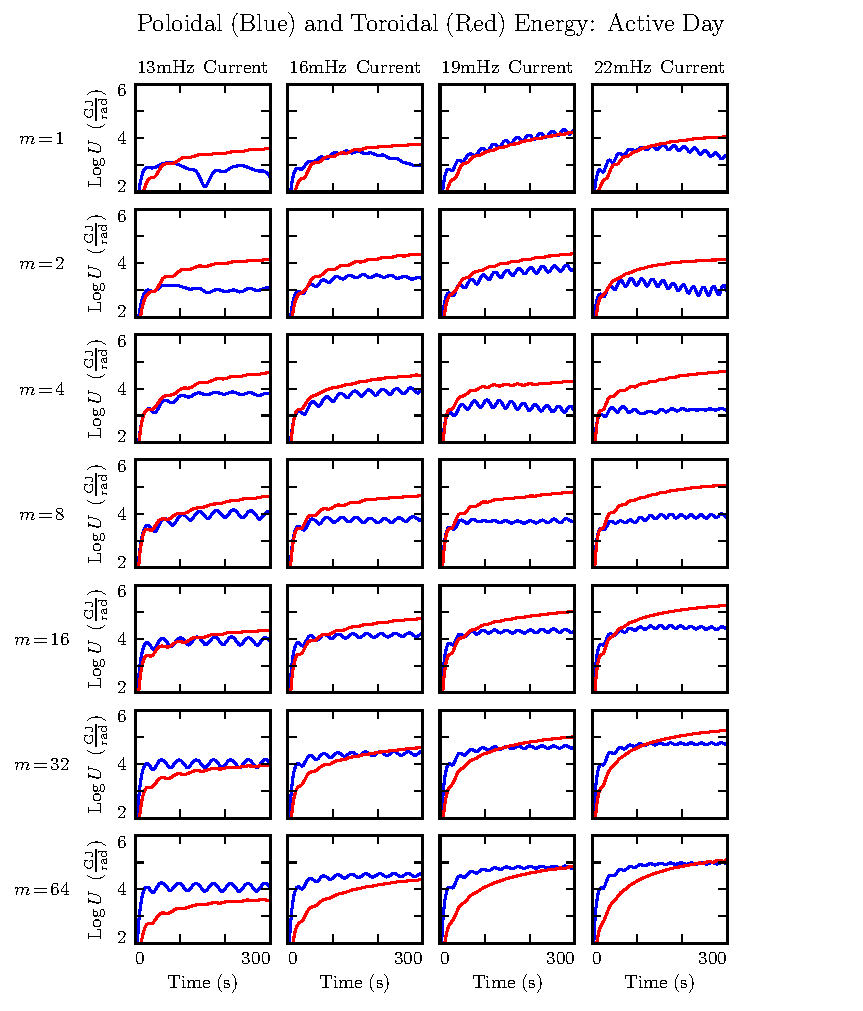
\includegraphics[width=\textwidth]{figures/U_1.pdf}
    \caption[Poloidal and Toroidal Energy: Active Day]{
      Driving is applied to the poloidal electric field. Over time, the energy rotates from the poloidal mode to the toroidal. The rotation rate is affected by the azimuthal modenumber. 
    }
    \label{fig_U_day}
\end{figure}

% -----------------------------------------------------------------------------
% -----------------------------------------------------------------------------
% -----------------------------------------------------------------------------
\subsection{Low Conductivity}

The picture on the nightside (where the ionospheric conductivity is low) is significantly different from the dayside (where it's high). 

Dissipation seems to outstrip rotation. Energy does not accumulate over numerous driving periods, as would be expected in resonance; it follows the driving up and down, as a damped-driven oscillator. 

There is evidence that the rotation is still trying to happen. At low \azm, energy is distributed between the poloidal and toroidal mode before dissipating; at high \azm, the energy dissipates straight out of the poloidal mode, never having had a chance to rotate. 

\begin{figure}[H]
    \centering
    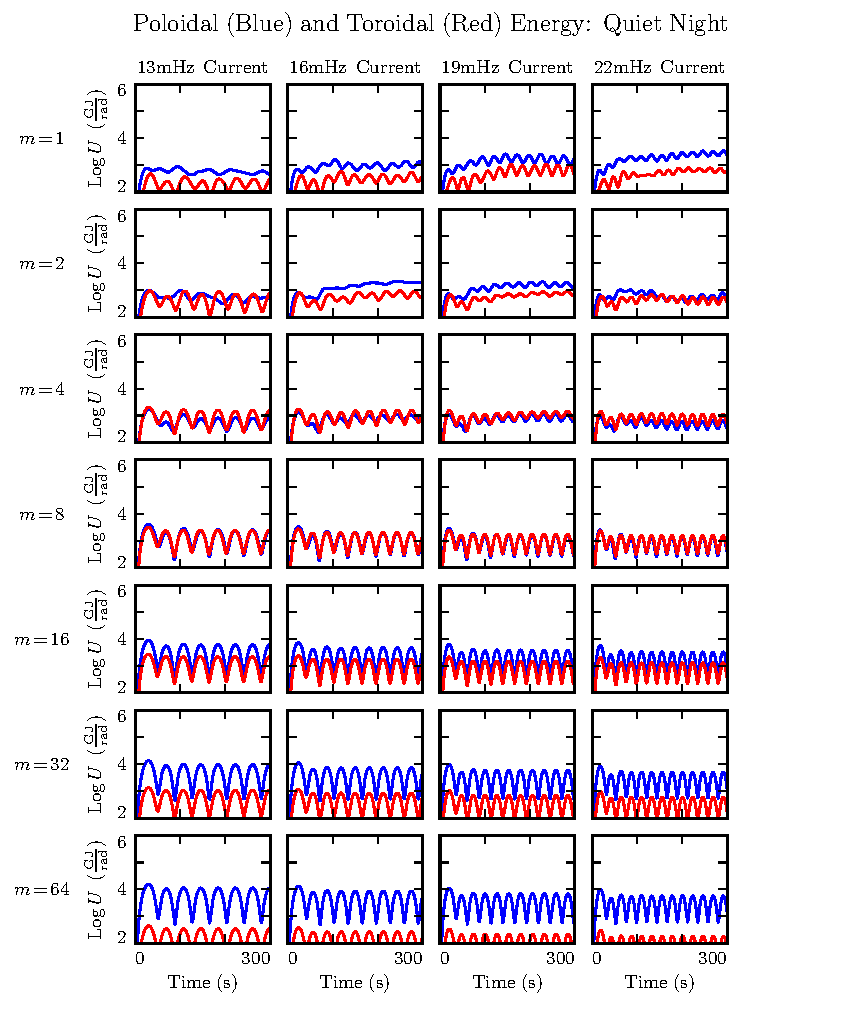
\includegraphics[width=\textwidth]{figures/U_4.pdf}
    \caption[Poloidal and Toroidal Energy: Quiet Night]{
      Driving is applied to the poloidal electric field. There is some rotation of energy to the toroidal mode (and less at high azimuthal modenumber), but the low ionospheric conductivity prevents energy from accumulating over time. 
    }
    \label{fig_U_night}
\end{figure}

% =============================================================================
% =============================================================================
% =============================================================================
\section{Spatial Distribution of Energy}
  \label{sec_shells}

Looking a bit deeper, it's possible to comment on the structure of the poloidal and toroidal modes, not just their magnitudes. The following commentary addresses the dayside; on the nightside, there's never much by the way of resonance. 

In \cref{fig_resonant_driving,fig_nonresonant_driving}, electromagnetic energy is binned by field line, averaged over volume (again, with respect to the Jacobian), and plotted as contours. All plots share a color scale. 

The poloidal mode and the toroidal mode exhibit qualitatively different behavior, related to the fact that energy rotates from poloidal to toroidal, and not back. 

At low \azm, energy rotates out of the poloidal mode so quickly that no resonance can form. 

At high \azm, the \Alfven wave is guided. If the driving frequency lines up with the resonant frequency where it's delivered, the poloidal mode resonates strongly. Otherwise, again, no energy accumulates. 

In no case does the poloidal mode demonstrate the ability to move energy across magnetic field lines. 

On the other hand, the toroidal mode does resonate, even if the driving isn't resonant (though in that case the response is of course stronger). The toroidal mode transports energy across field lines until it encounters resonance, then accumulates energy there. Often, resonances are seen in multiple locations due to the non-monotonic \Alfven bounce frequency (recall \cref{fig_fa}) as a function of $L$. 

% -----------------------------------------------------------------------------
% -----------------------------------------------------------------------------
% -----------------------------------------------------------------------------
\subsection{Resonant Driving}

\begin{figure}[H]
    \centering
    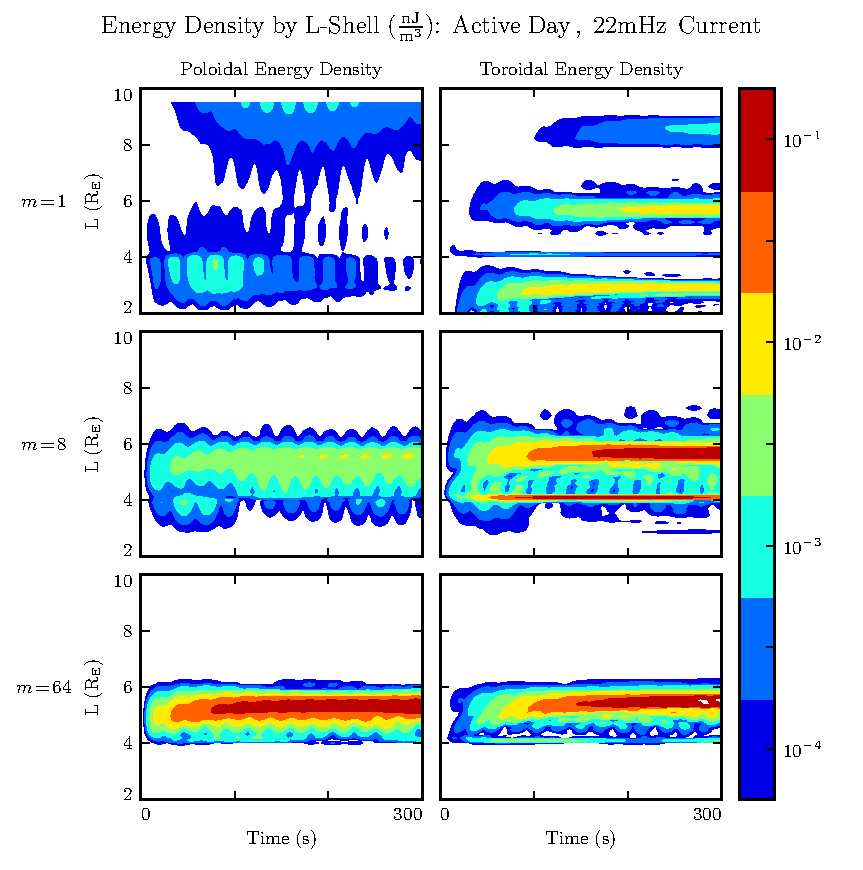
\includegraphics[width=\textwidth]{figures/layers_22mHz_1.pdf}
    \caption[Poloidal and Toroidal Energy Distribution: Resonant Driving]{
      If \azm is small, energy rotates to the toroidal mode too fast to form a poloidal resonance. If \azm is large, the \Alfven wave is guided, so it resonates only if the driving frequency lines up with the resonant frequency where it's applied. The result is just one big -- or perhaps even giant -- pulsation. If the driving lines up with a nearby field line, the toroidal mode goes crazy! Resonance inside the plasmasphere. Resonance at the plasmapause. Resonance at the driving location. And (weak) attempt at a higher harmonic further out. 
    }
    \label{fig_resonant_driving}
\end{figure}

% -----------------------------------------------------------------------------
% -----------------------------------------------------------------------------
% -----------------------------------------------------------------------------
\subsection{Nonresonant Driving}

\begin{figure}[H]
    \centering
    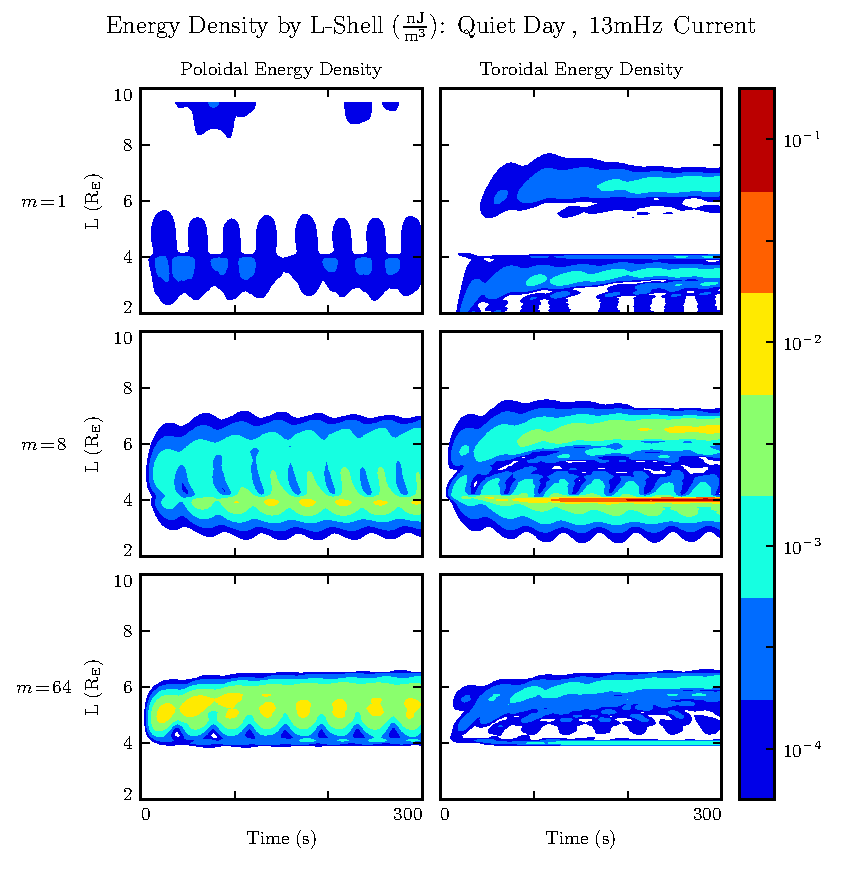
\includegraphics[width=\textwidth]{figures/layers_13mHz_2.pdf}
    \caption[Poloidal and Toroidal Energy Distribution: Nonresonant Driving]{
      When the driving frequency doesn't line up with the location where it's delivered, there's basically no response. There is no movement of energy to a resonant field line, so no energy can accumulate over the course of multiple rounds of driving. Even when not driven resonantly, the toroidal mode still makes the best of its situation. It steals what energy it can from the poloidal mode, carries it to the resonant $L$-shell, and gets to work. (In contrast, recall from \cref{fig_resonant_driving}, in this situation the poloidal mode just does not accumulate energy.)
    }
    \label{fig_nonresonant_driving}
\end{figure}

% =============================================================================
% =============================================================================
% =============================================================================
\section{Significance for Giant Pulsations}

Giant pulsations are (probably\cite{takahashi_2011}) fundamental mode poloidal Pc4 pulsations with frequencies around \SI{10}{\mHz} and azimuthal modenumbers around \num{20}. They are large, and can sometimes be observed on the ground. 

While this model makes no particular distinction between a giant pulsation and any other Pc4, the above results do line up with giant pulsation observations. 

Giant pulsations aren't seen at small \azm. As shown in \cref{sec_lifetimes}, low-\azm poloidal modes rotate to the toroidal mode too quickly to resonate effectively, even in the case of continuous driving at a locally-resonant frequency. The sweet spot seems to be around $\azm = 20$, more or less the same point where resonance becomes visible in \cref{fig_resonant_driving}. Admittedly, giant pulsations are typically closer to \SI{10}{\mHz} than \SI{22}{\mHz}. It seems likely that qualitatively similar results would be encountered if the driving were moved to an $L$-shell with a bounce time of \SI{10}{\mHz}. 

Giant pulsations are seen at very large \azm, though not on the ground\cite{takahashi_2013}, due to damping by the ionosphere. 

Giant pulsations are most common on the dayside (particularly the morningside), during geomagnetically quiet times. Giant pulsation ground signatures are noted for their predisposition towards east-west polarization. 

In \cref{fig_ground_signatures}, the strongest east-west ground signatures is obtained on the geomagnetically quiet dayside, at \azm of 16 and 32. 

This seems to be a giant pulsation ``sweet spot'': the poloidal mode becomes stronger as \azm increases, but the ionospheric damping also increases. 

% -----------------------------------------------------------------------------
% -----------------------------------------------------------------------------
% -----------------------------------------------------------------------------
\subsection{Ground Signatures}

\begin{figure}[H]
    \centering
    \includegraphics[width=\textwidth]{figures/ground_16mHz.pdf}
    \caption[Dayside Ground Magnetic Fields]{
      The east-west component of magnetic ground signatures is peaked on the geomagnetically quiet dayside, at modenumbers around 16 to 32. This coincides nicely with observations of giant pulsations. Like the east-west component, the north-south ground signature is strongest on the quiet dayside; however, unlike the east-west component, the north-south component is weak when the modenumber is large. 
    }
    \label{fig_ground_signatures}
\end{figure}

Giant pulsations are monochromatic, and can be accompanied by ``multiharmonic toroidal waves''\cite{takahashi_2011}. Per \cref{sec_shells}, this is about what would be expected from a mishmash of poloidal driving. Poloidal modes of all frequencies rotate into the toroidal mode; resonant poloidal modes resonate; non-resonant poloidal modes become evanescent. 

Giant pulsations often drift azimuthally. This model can't resolve azimuthal drift directly, of course, but can fake it by looking at complex phase. There has been some indication (not shown) of complex phase rotation in ground magnetic fields. However, at the boundary, it's difficult to disentangle which values are imaginary to indicate an azimuthal offset, and which are imaginary because of Hall coupling. Investigation is ongoing. 


% =============================================================================
% =============================================================================
% =============================================================================
%\section{Electromagnetic Energy Gap}

%\todo{A preliminary search (and asking Bob) has not turned up anyone looking at this before, so it's hard to provide context. }

%Above, we considered the decay of energy from the poloidal mode to the toroidal mode. A natural follow up is, are there any other surprising trends in the distribution of energy?

%As it turns out, yes!

%In cases where the driving frequency does not line up with the local bounce frequency, energy doesn't accumulate particularly well in either the poloidal or the toroidal mode. Like a damped-driven oscillator, the system's behavior follows the input. 

%At low \azm, what energy there is divides itself more-or-less equally between the electric and magnetic fields. 

%As \azm increases, oddly, a gap appears. When the conductivity is high, the magnetic field holds more energy than the electric field. The disparity can be up to a factor of $\sim \num{3}$; that is, \SI{75}{\percent}. of the energy in the magnetic field, and \SI{25}{\percent} in the electric field. When conductivity is low, the opposite happens: energy concentrates in the electric field. 

%This lines up somewhat with what might be expected. When conductivity is low, it takes a larger electric field to induce the same current, and thus the same magnetic field. But it's not clear why this disparity only appears at large \azm, or why it does not appear when the driving is resonant. 

%Maybe it's a timing issue? A relationship between the bounce time (which is more or less indepedent of \azm) and the rotation time (which depends on \azm). 

%\todo{How is the compressional magnetic field brought into these calculations? It exists only at small \azm. It's never particularly large, it also gets added to the zeroth-order field before squaring. }

%\begin{figure}[H]
%    \centering
%    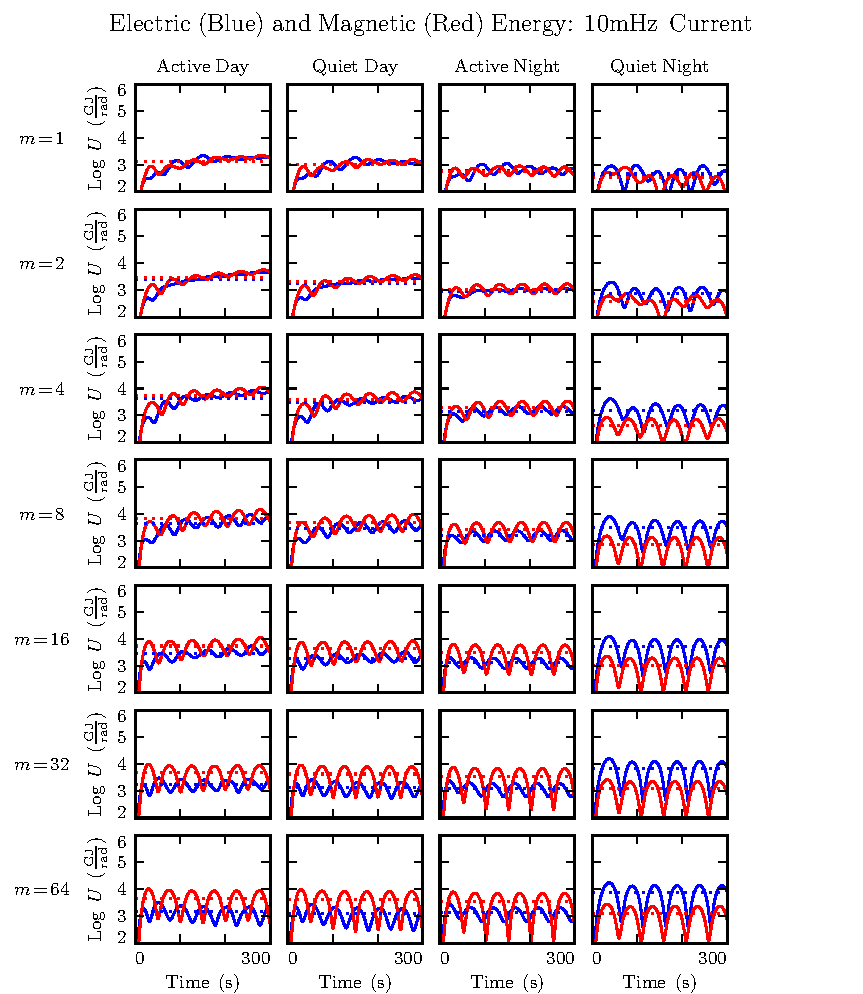
\includegraphics[width=\textwidth]{figures/U_BE_010mHz.pdf}
%    \caption[Current-Driven Electric and Magnetic Energy: 10mHz]{
%      In the absence of resonant driving, a disparity emerges at large \azm between the energy in the magnetic field and the energy in the electric field. The sign of the difference depends on the ionospheric conductivity. 
%    }
%    \label{fig_U_BE_010mHz}
%\end{figure}

%\begin{figure}[H]
%    \centering
%    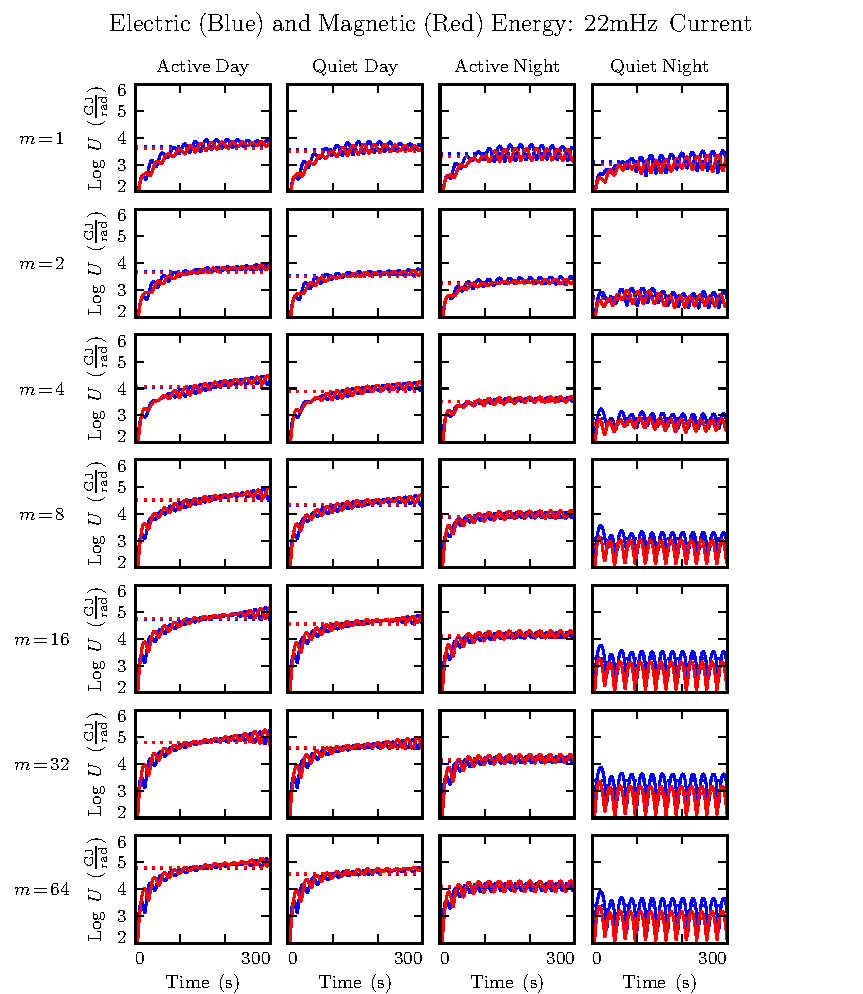
\includegraphics[width=\textwidth]{figures/U_BE_022mHz.pdf}
%    \caption[Current-Driven Electric and Magnetic Energy: 22mHz]{
%      When driving is resonant, energy is distributed almost exactly half-and-half between the electric and magnetic fields, regardless of \azm. The rightmost profile still shows a gap, likely because the ionospheric conductivity in that model is low enough that nothing ever resonates. 
%    }
%    \label{fig_U_BE_022mHz}
%\end{figure}












